\documentclass[tikz, border=10pt]{standalone}
\usepackage{tikz}
\usepackage{amsmath}
\usepackage{xcolor}
\usetikzlibrary{arrows.meta}

\begin{document}
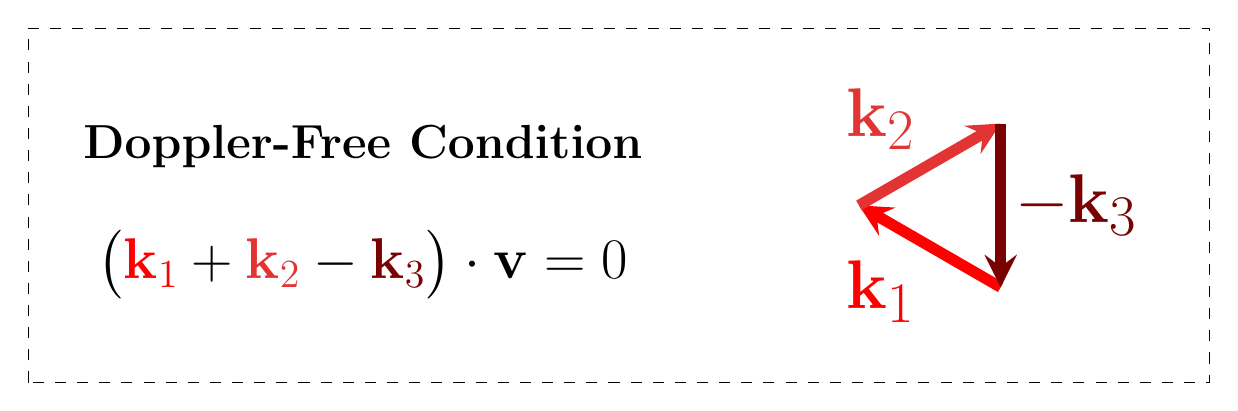
\begin{tikzpicture}

% =======================================================
% Color definitions (wavelength-labeled)
% =======================================================
\definecolor{c689}{HTML}{FF0000}   % beam 1 (689 nm)
\definecolor{c688}{HTML}{E33434}   % beam 2 (688 nm)
\definecolor{c679}{HTML}{780202}   % beam 3 (679 nm)

% =======================================================
% Layout parameters
% =======================================================

% k-vector triangle radius
\def\rad{1.2}

% Dashed bounding box dimensions
\def\boxx{15}
\def\boxy{5}
\def\boxvspace{-0.5}   % vertical trim on top edge

% =======================================================
% Styles
% =======================================================
\tikzset{
  kvec/.style = {ultra thick, ->, >=stealth, line width=4, font=\Huge},
}

% % =======================================================
% % Doppler-free condition square
% % =======================================================

% % Triangle vertices at 120-degree spacing
% \coordinate (A) at ({\rad*cos(-60)},  {\rad*sin(-60)});   % bottom-right
% \coordinate (B) at ({\rad*cos(-180)}, {\rad*sin(-180)});   % left
% \coordinate (C) at ({\rad*cos(60)},   {\rad*sin(60)});     % top-right

% % k_1: bottom-right -> left
% \draw[c689, kvec] (A) -- (B) node[midway, below left]  {$\mathbf{k}_1$};

% % k_2: left -> top-right
% \draw[c688, kvec] (B) -- (C) node[midway, above left]  {$\mathbf{k}_2$};

% % -k_3: top-right -> bottom-right (closes the triangle)
% \draw[c679, kvec] (C) -- (A) node[midway, right]       {$-\mathbf{k}_3$};

% % Dashed border
% \draw[dash pattern=on 12pt off 4pt, ultra thick]
%   (-\boxx/2, -\boxy/2) rectangle ++(\boxx, \boxy+\boxvspace);

% % Title
% \node[black, above, font=\bfseries\LARGE]
%   at (0, \boxy/2 - 1.3) {Doppler-Free Condition};

% % Phase-matching equation
% \node[black, above, font=\huge]
%   at (0, -\boxy/2 + 0.1)
%   {$\bigl(\textcolor{c689}{\mathbf{k}_1}
%     + \textcolor{c688}{\mathbf{k}_2}
%     - \textcolor{c679}{\mathbf{k}_3}\bigr)
%     \cdot \mathbf{v} = 0$};


  % =======================================================
% Doppler-free condition bod rectangular
% =======================================================

% Title
\node[black, font=\bfseries\LARGE, align=center]
    at (-4.5, 0.75)
    {Doppler-Free Condition};

% Main Doppler condition
\node[black, font=\huge]
    at (-4.5, -0.75)
    {$\bigl(
    \textcolor{c689}{\mathbf{k}_1}
    +\textcolor{c688}{\mathbf{k}_2}
    -\textcolor{c679}{\mathbf{k}_3}
    \bigr)\cdot \mathbf{v}=0$};

% Right side: wave-vector triangle

\begin{scope}[shift={(3.0,0)}]

% Triangle vertices at 120-degree spacing
\coordinate (A) at ({\rad*cos(-60)},  {\rad*sin(-60)});   % bottom-right
\coordinate (B) at ({\rad*cos(-180)}, {\rad*sin(-180)});  % left
\coordinate (C) at ({\rad*cos(60)},   {\rad*sin(60)});    % top-right

% k_1: bottom-right -> left
\draw[c689, kvec]
    (A) -- (B)
    node[midway, below left] {$\mathbf{k}_1$};

% k_2: left -> top-right
\draw[c688, kvec]
    (B) -- (C)
    node[midway, above left] {$\mathbf{k}_2$};

% -k_3: top-right -> bottom-right
\draw[c679, kvec]
    (C) -- (A)
    node[midway, right] {$-\mathbf{k}_3$};

\end{scope}

\begin{scope}[shift={(-1.25,0.25)}]

\draw[dash pattern=on 4pt off 4pt, thin]
   (-\boxx/2, -\boxy/2) rectangle ++(\boxx, \boxy+\boxvspace);
\end{scope}

%%%%%%%%%%%%%%%%%%%%%%%%%%%%%%%%%%%%%%%%%%%%%%%%%%%%%%%%

\end{tikzpicture}
\end{document}